%%%%%%%%%%%%%%%%%%%%%%%%%%%%%%%%%%%%%%%%%
% Beamer Presentation
% LaTeX Template
% Version 1.0 (10/11/12)
%
% This template has been downloaded from:
% http://www.LaTeXTemplates.com
%
% License:
% CC BY-NC-SA 3.0 (http://creativecommons.org/licenses/by-nc-sa/3.0/)
%
%%%%%%%%%%%%%%%%%%%%%%%%%%%%%%%%%%%%%%%%%

%----------------------------------------------------------------------------------------
%	PACKAGES AND THEMES
%----------------------------------------------------------------------------------------

\documentclass{beamer}

\mode<presentation> {

% The Beamer class comes with a number of default slide themes
% which change the colors and layouts of slides. Below this is a list
% of all the themes, uncomment each in turn to see what they look like.

%\usetheme{default}
%\usetheme{AnnArbor}
%\usetheme{Antibes}
%\usetheme{Bergen}
%\usetheme{Berkeley}
%\usetheme{Berlin}
%\usetheme{Boadilla}
%\usetheme{CambridgeUS}
%\usetheme{Copenhagen}
%\usetheme{Darmstadt}
%\usetheme{Dresden}
%\usetheme{Frankfurt}
%\usetheme{Goettingen}
%\usetheme{Hannover}
%\usetheme{Ilmenau}
%\usetheme{JuanLesPins}
%\usetheme{Luebeck}
\usetheme{Madrid}
%\usetheme{Malmoe}
%\usetheme{Marburg}
%\usetheme{Montpellier}
%\usetheme{PaloAlto}
%\usetheme{Pittsburgh}
%\usetheme{Rochester}
%\usetheme{Singapore}
%\usetheme{Szeged}
%\usetheme{Warsaw}

% As well as themes, the Beamer class has a number of color themes
% for any slide theme. Uncomment each of these in turn to see how it
% changes the colors of your current slide theme.

%\usecolortheme{albatross}
%\usecolortheme{beaver}
%\usecolortheme{beetle}
%\usecolortheme{crane}
%\usecolortheme{dolphin}
%\usecolortheme{dove}
%\usecolortheme{fly}
%\usecolortheme{lily}
%\usecolortheme{orchid}
%\usecolortheme{rose}
%\usecolortheme{seagull}
%\usecolortheme{seahorse}
\usecolortheme{whale}
%\usecolortheme{wolverine}

%\setbeamertemplate{footline} % To remove the footer line in all slides uncomment this line
%\setbeamertemplate{footline}[page number] % To replace the footer line in all slides with a simple slide count uncomment this line

\setbeamertemplate{navigation symbols}{} % To remove the navigation symbols from the bottom of all slides uncomment this line
}
\usepackage[T1]{fontenc}

\usepackage{graphicx} % Allows including images
\DeclareGraphicsExtensions{.pdf,.png,.jpg}
\usepackage{booktabs} % Allows the use of \toprule, \midrule and \bottomrule in tables
\usepackage[skip = 2pt, font=scriptsize]{caption}
\usepackage{subfigure}

%----------------------------------------------------------------------------------------
%	TITLE PAGE
%----------------------------------------------------------------------------------------

\title[Master Thesis]{Implementation of Monte Carlo fitter and Selection of $B \rightarrow K^* \mu \mu$ decays in LHCb Run2 data.} % The short title appears at the bottom of every slide, the full title is only on the title page

\author{Oliver Dahme} % Your name
\institute[UZH] % Your institution as it will appear on the bottom of every slide, may be shorthand to save space
{
University of Zurich \\ % Your institution for the title page
\medskip
\textit{o.dahme@cern.ch} % Your email address
}
\date{\today} % Date, can be changed to a custom date

\begin{document}

\begin{frame}
 \titlepage % Print the title page as the first slide
 \centering Supervisors: Prof. Dr. Nicola Serra, Prof. Dr. Marcin Chrzs\k{a}szcz
\end{frame}

\begin{frame}
 \frametitle{Overview} % Table of contents slide, comment this block out to remove it
 \tableofcontents % Throughout your presentation, if you choose to use \section{} and \subsection{} commands, these will automatically be printed on this slide as an overview of your presentation
\end{frame}

%----------------------------------------------------------------------------------------
%	PRESENTATION SLIDES
%----------------------------------------------------------------------------------------


\section{LHCb Detector}

\begin{frame}
  \frametitle{The LHCb Detector}

  \begin{figure}
    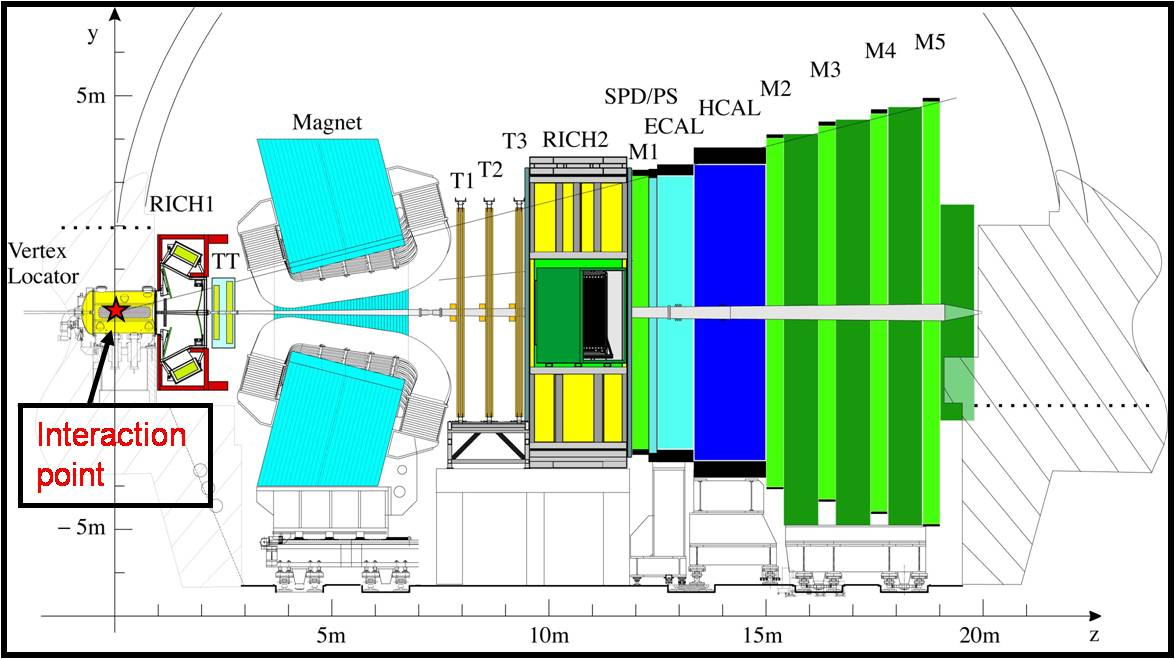
\includegraphics[width=1.0\linewidth]{figures/lhcb_detector}
    \caption{Detector overview}
      % a lot of talking about the different components and their functions
  \end{figure}

\end{frame}

%------------------------------------------------------------------------------



%------------------------------------------------------------------------------

\section{The $B_0 \rightarrow K^* \mu^+ \mu^-$ decay }

\begin{frame}
  \frametitle{The $B_0 \rightarrow K^* \mu^+ \mu^-$ decay}

  \begin{figure}[H]
 \centering
 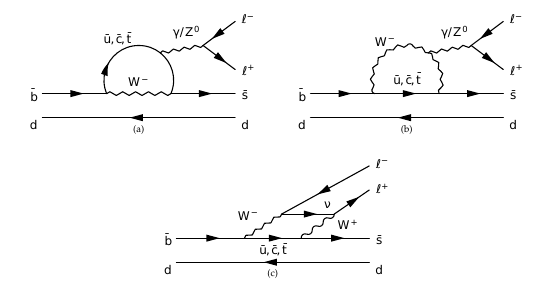
\includegraphics[width=0.8\linewidth]{figures/KstarFeynman}
 \caption{Feynman diagrams for decay $B(\bar{b},d)$ $\rightarrow$ $ K^*(\bar{s},d) l^+$ $l^-$ at lowest order}
 \label{fig:Feynman}
\end{figure}

\end{frame}

\begin{frame}
  \frametitle{Variables defining the decay}

The kinematics and directions of the final state particles from the decay are defined by the three angels $\theta_K$, $\theta_L$ and $\phi$ and the invariant di-muon mass square $q^2$.

  \begin{figure}
   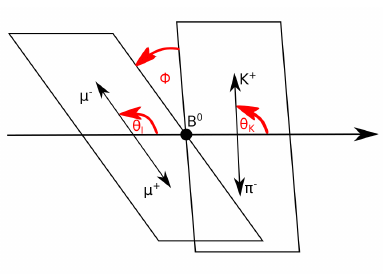
\includegraphics[width= 0.8\linewidth]{figures/angels}
   \caption{Angels defining the decay $B^0$ $\rightarrow$ $K^{*0}$ $\mu$ $\mu$}
  \end{figure}

\end{frame}


\begin{frame}
  \frametitle{Motivation}

Recent experimental results of the LHCb collaboration [JHEP08 (2017) 055] suggest a violation of the lepton universality:

  \begin{equation}
\begin{split}
R_{K*0} &= \left. \dfrac{\mathcal{B}(B^0 \rightarrow K^{*0} \mu^+ \mu^-)}{\mathcal{B}(B^0 \rightarrow K^{*0} J/\psi(\rightarrow \mu^+ \mu^-))} \middle/   \dfrac{\mathcal{B}(B^0 \rightarrow K^{*0} e^+ e^-)}{\mathcal{B} ( B^0 \rightarrow K^{*0} J/\psi(\rightarrow e^+ e^-))}  \right. , \\
R_{K*0} &=   \begin{cases}
  0.66^{+0.11}_{-0.07} (\text{stat}) \pm 0.03 (\text{syst}) \text{ for } 0.045 < q^2 < 1.1 \text{ GeV}^2/c^4, \\
  0.69^{+0.11}_{-0.07} (\text{stat}) \pm 0.05 (\text{syst}) \text{ for } 1.1 < q^2 < 6.0 \text{ GeV}^2/c^4.
\end{cases}
\end{split}
\end{equation}

\end{frame}



%------------------------------------------------------------------------------

\section{Selection of $B_0 \rightarrow K^* \mu^+ \mu^-$ decays}



\begin{frame}
  \frametitle{Decision tree}

Decision trees are structured in Nodes, which represent the input features and in Leaves, which can be seen as terminal nodes.

  \begin{figure}
   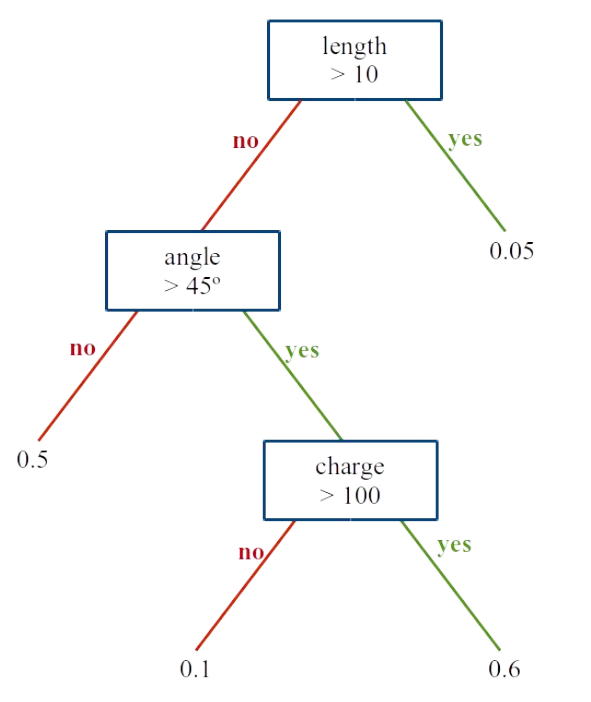
\includegraphics[width=0.5\textwidth]{figures/decision_tree}
   \caption{Example of a decision tree.}
   \label{fig:tree}
  \end{figure}
\end{frame}



\begin{frame}
  \frametitle{Selection of $B_0 \rightarrow K^* \mu^+ \mu^-$ decays}

To select the decay from the raw Run2 data, boost decision trees and the K-folding technique were used. To find the best boost decision tree algorithm, the following were tested:

\begin{itemize}
 \item Ada Boost
 \item uGB  + knnAda (k-nearest neghbor AdaBoost)
 \item uBoost
 \item uGB  + Fl (flatness loss)
 \item xgb
 \item sk\_bdtg
 \item sk\_bdt
\end{itemize}

\end{frame}


%------------------------------------------------------------------------------

\begin{frame}
  \frametitle{Selection of $B_0 \rightarrow K^* \mu^+ \mu^-$ decays}

  \begin{figure}
   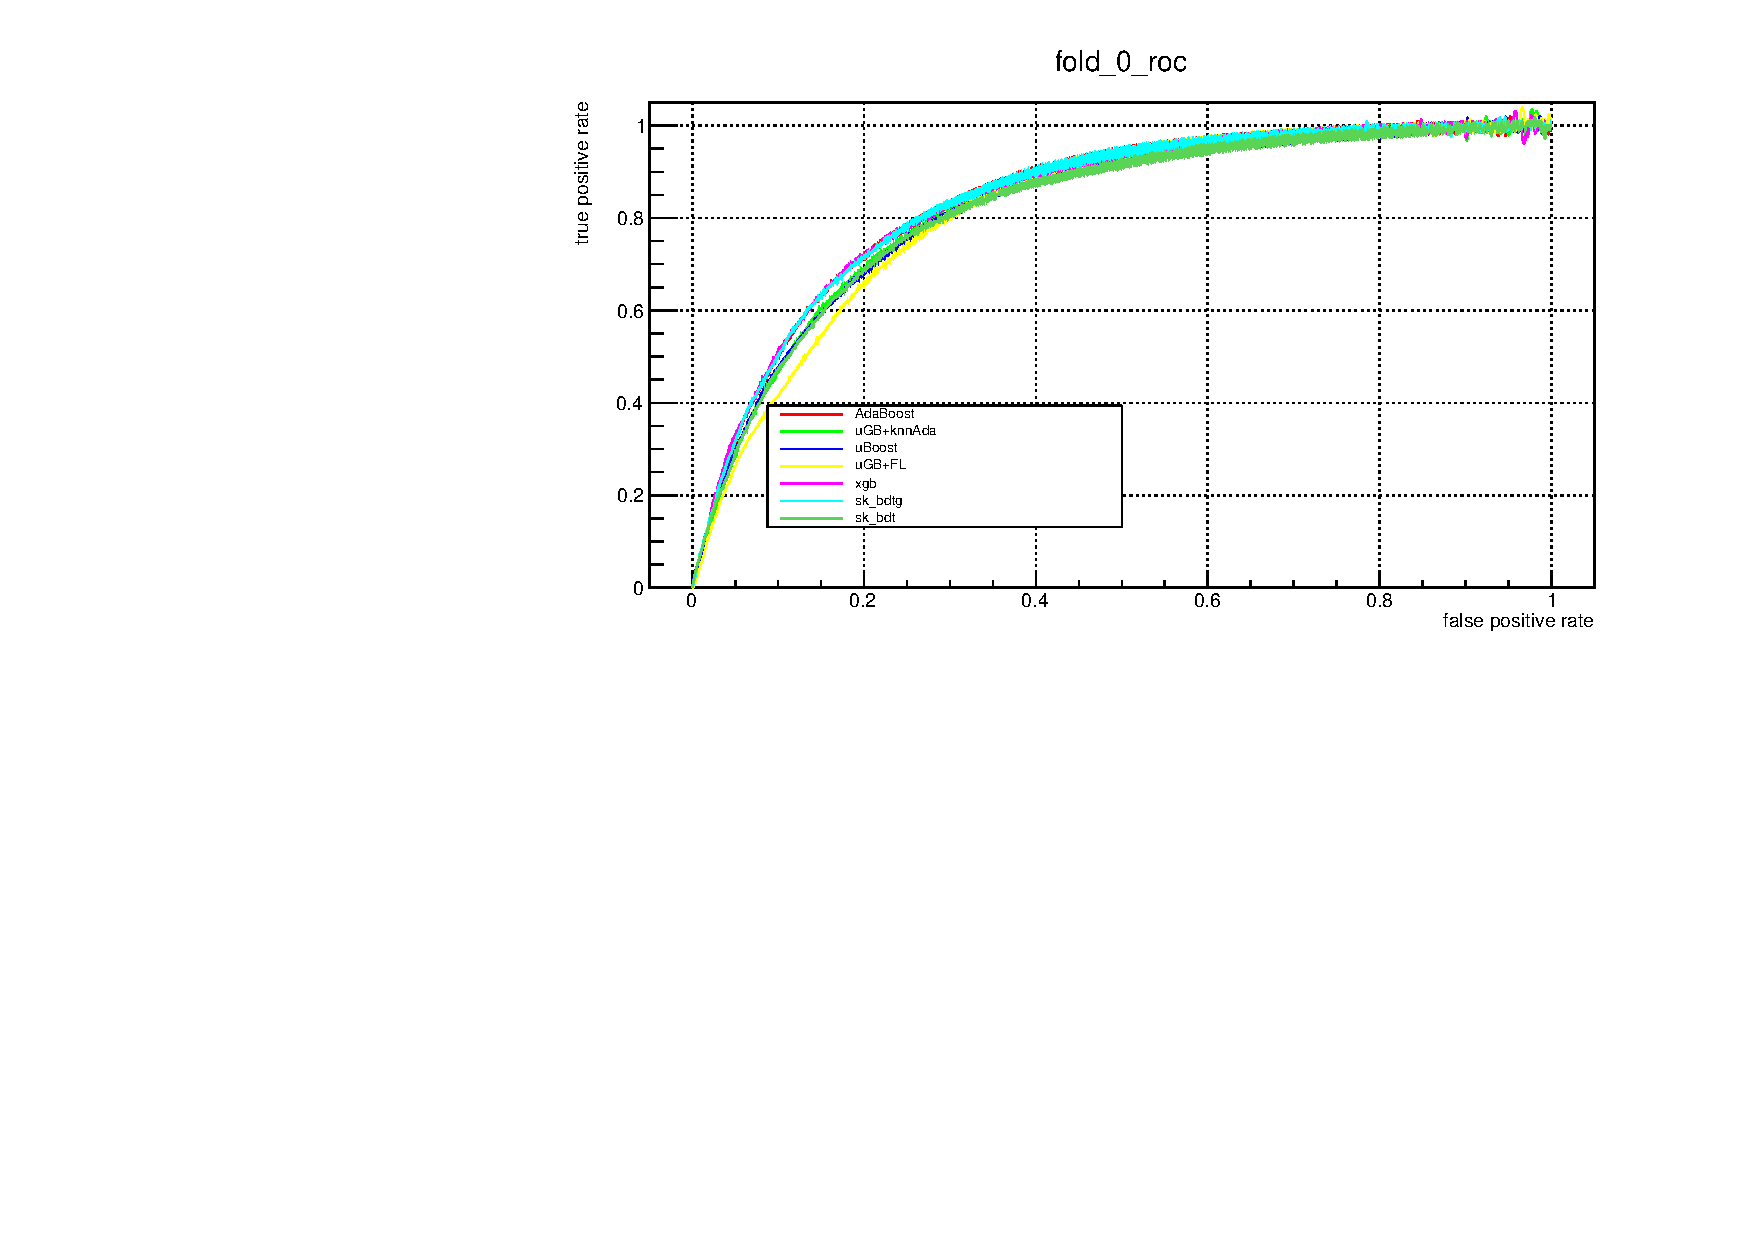
\includegraphics[width= 1.0\linewidth]{figures/roc}
   \caption{ROC (receiver operating charactertic) curve}
  \end{figure}

\end{frame}


%------------------------------------------------------------------------------

\begin{frame}
  \frametitle{Selection of $B_0 \rightarrow K^* \mu^+ \mu^-$ decays}

  \begin{figure}
   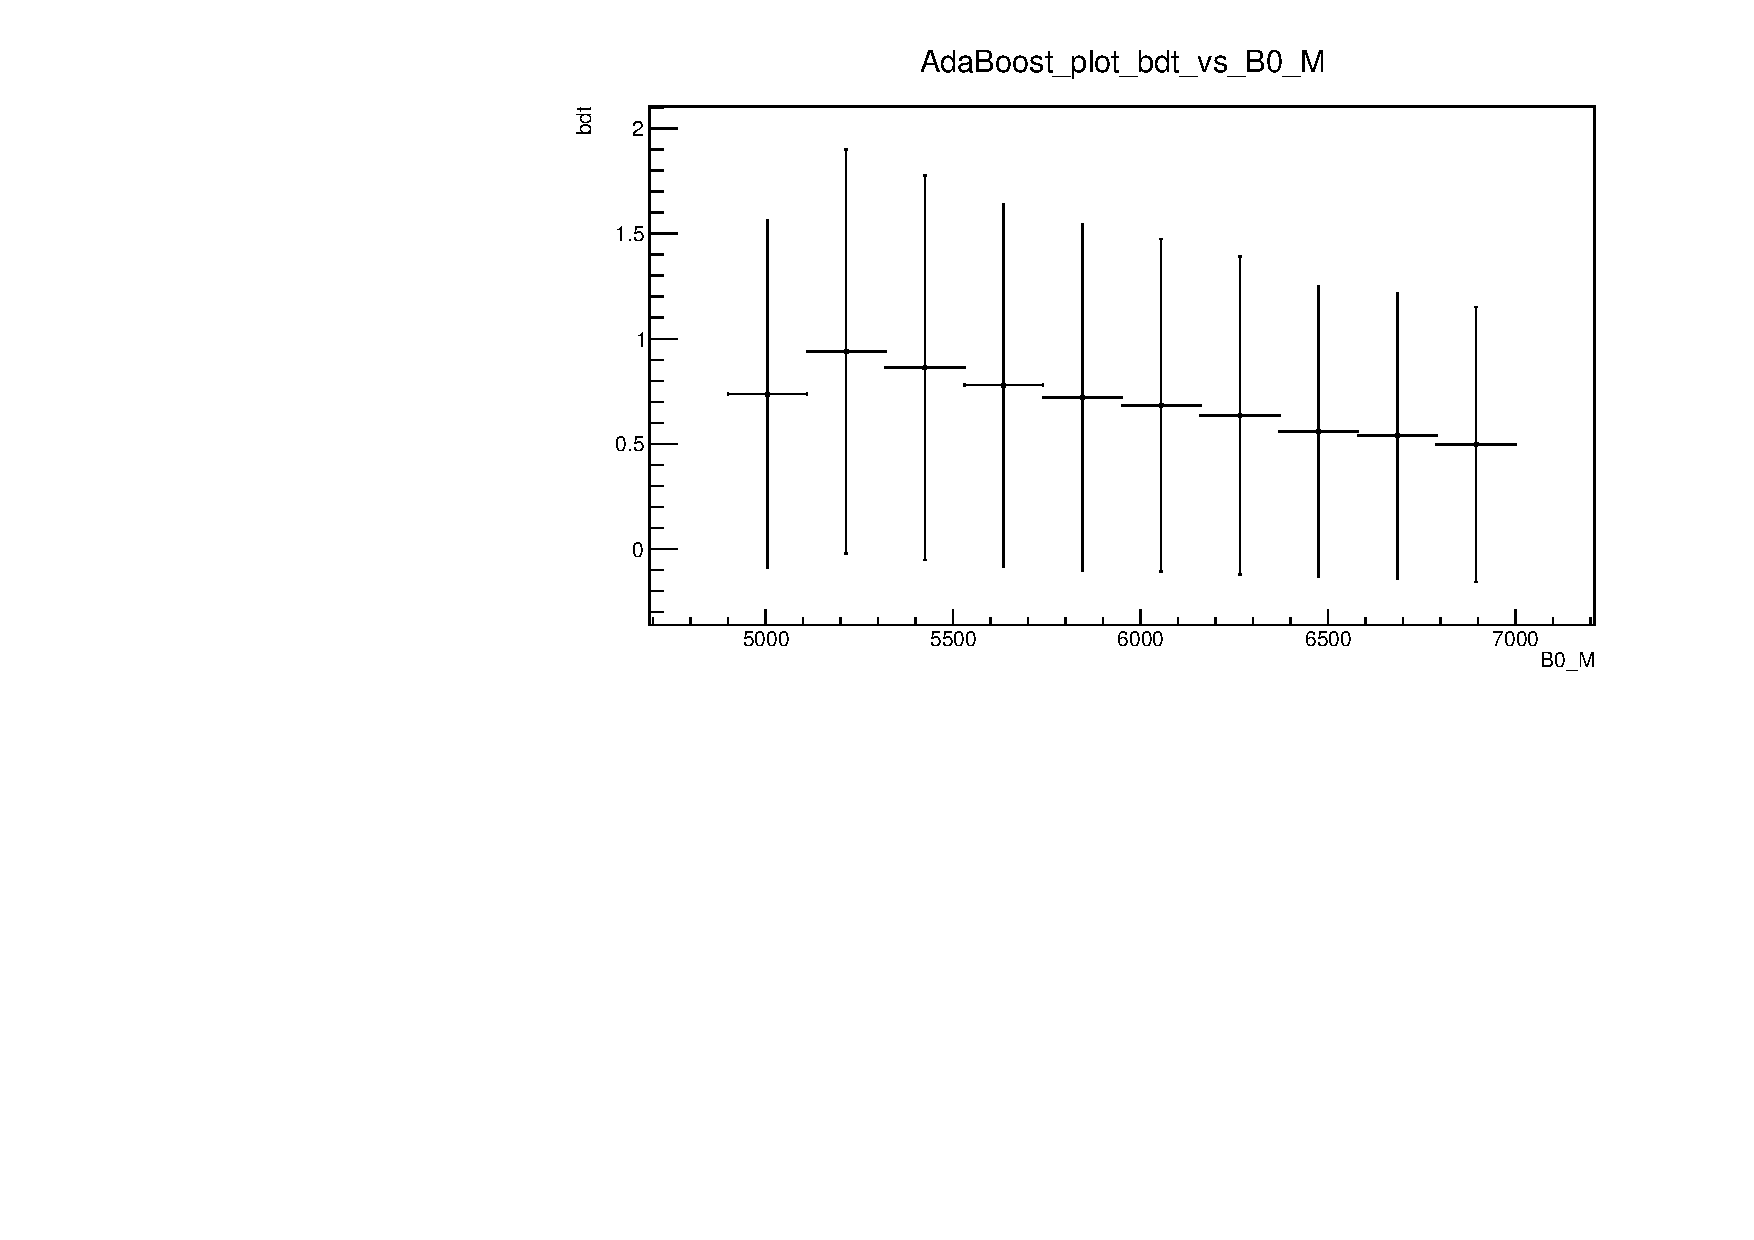
\includegraphics[width=0.8\linewidth]{figures/cor_AdaBoost}
   \caption{Correlation plot between $B$ mass in Mev and the response of the AdaBoost algorithm.}
  \end{figure}

\end{frame}


%------------------------------------------------------------------------------

\begin{frame}
  \frametitle{Selection of $B_0 \rightarrow K^* \mu^+ \mu^-$ decays}

  \begin{figure}
   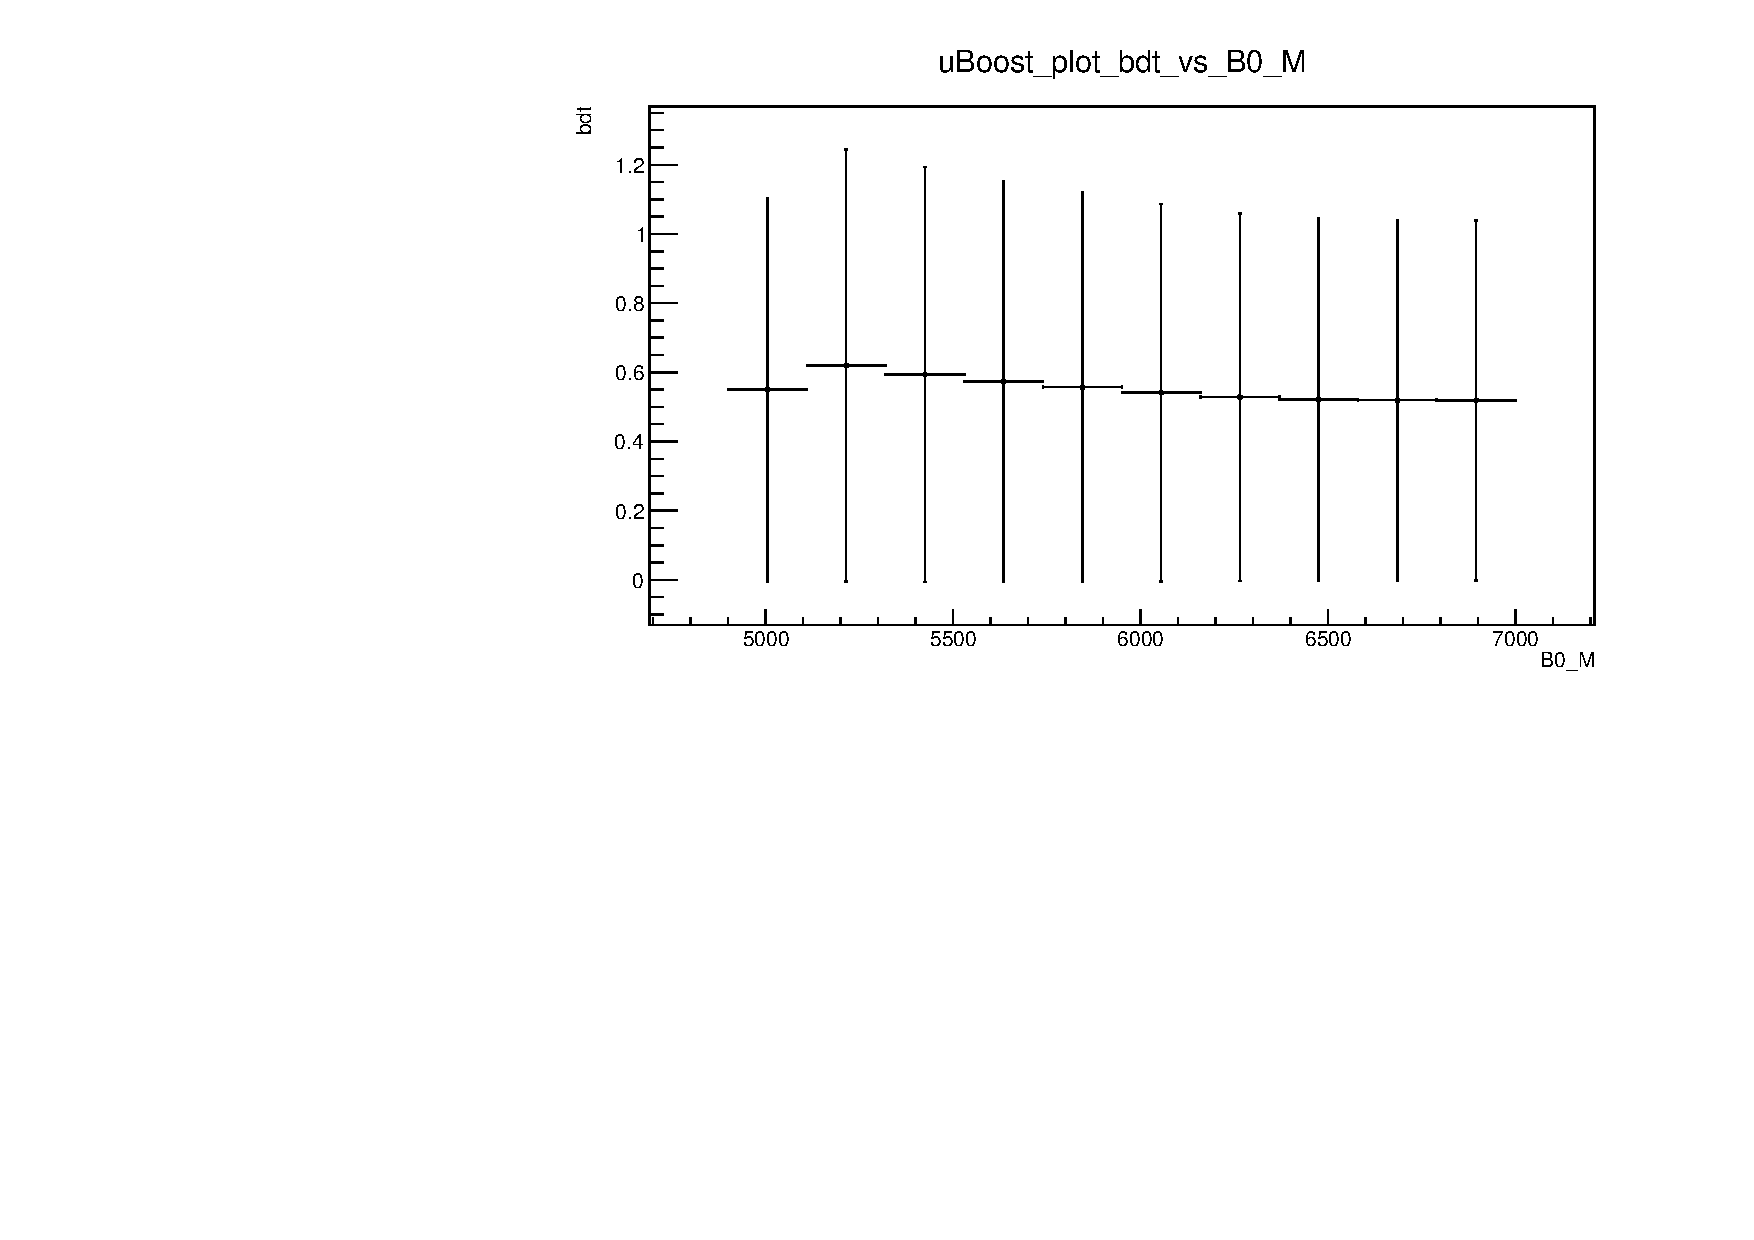
\includegraphics[width=0.8\linewidth]{figures/cor_uBoost}
   \caption{Correlation plot between $B$ mass in Mev and the response of the uBoost algorithm.}
  \end{figure}

\end{frame}


%------------------------------------------------------------------------------

\section{Reweighting}

\begin{frame}
  \frametitle{Reweighting}

    \begin{itemize}
      \item procedure to match Monte Carlo simulation to data
      \item get detector efficiencies
      \item done by applying weights to the MC events
      \item choosen be comparing MC and data
    \end{itemize}
compare parameters:
\begin{itemize}
  \item number of Tracks
  \item the quality of the $K \pi \mu \mu$ vertex
  \item transversal momentum of the $B$ meson
\end{itemize}

\end{frame}

\begin{frame}
  \frametitle{Reweighting}

  \begin{figure}
   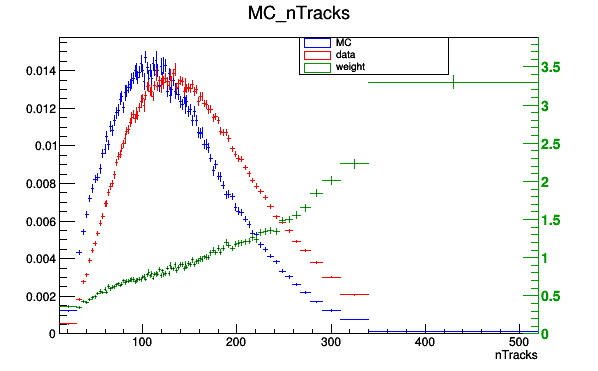
\includegraphics[width=0.8\linewidth]{figures/nTracksw}
   \caption{Reweighting result for the number of tracks}
  \end{figure}


\end{frame}

%------------------------------------------------------------------------------

\begin{frame}
  \frametitle{Reweighting}

  \begin{figure}
   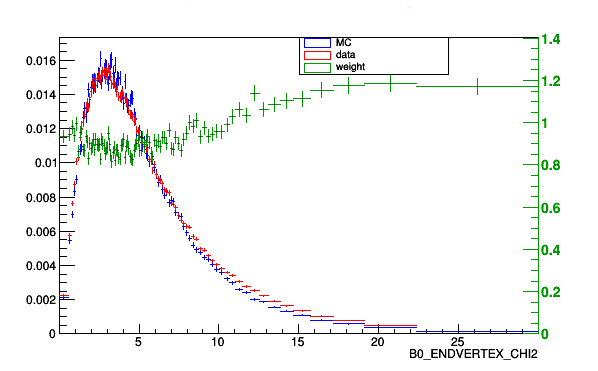
\includegraphics[width=0.8\linewidth]{figures/B0_ENDVERTEX_CHI2w}
   \caption{Reweighting result for the quality of the $K \pi \mu \mu$ vertex (B0\_ENDVERTEX\_CHI2)}
  \end{figure}


\end{frame}

%------------------------------------------------------------------------------

\begin{frame}
  \frametitle{Reweighting}

  \begin{figure}
   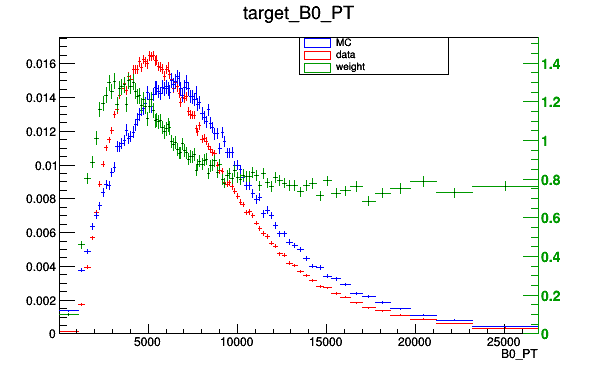
\includegraphics[width=0.8\linewidth]{figures/B0_PTw}
   \caption{Reweighting result for the transversal momentum of the $B$ meson (B0\_PT) in MeV.}
  \end{figure}


\end{frame}

%------------------------------------------------------------------------------

\begin{frame}
  \frametitle{Reweighting}

  \begin{figure}
   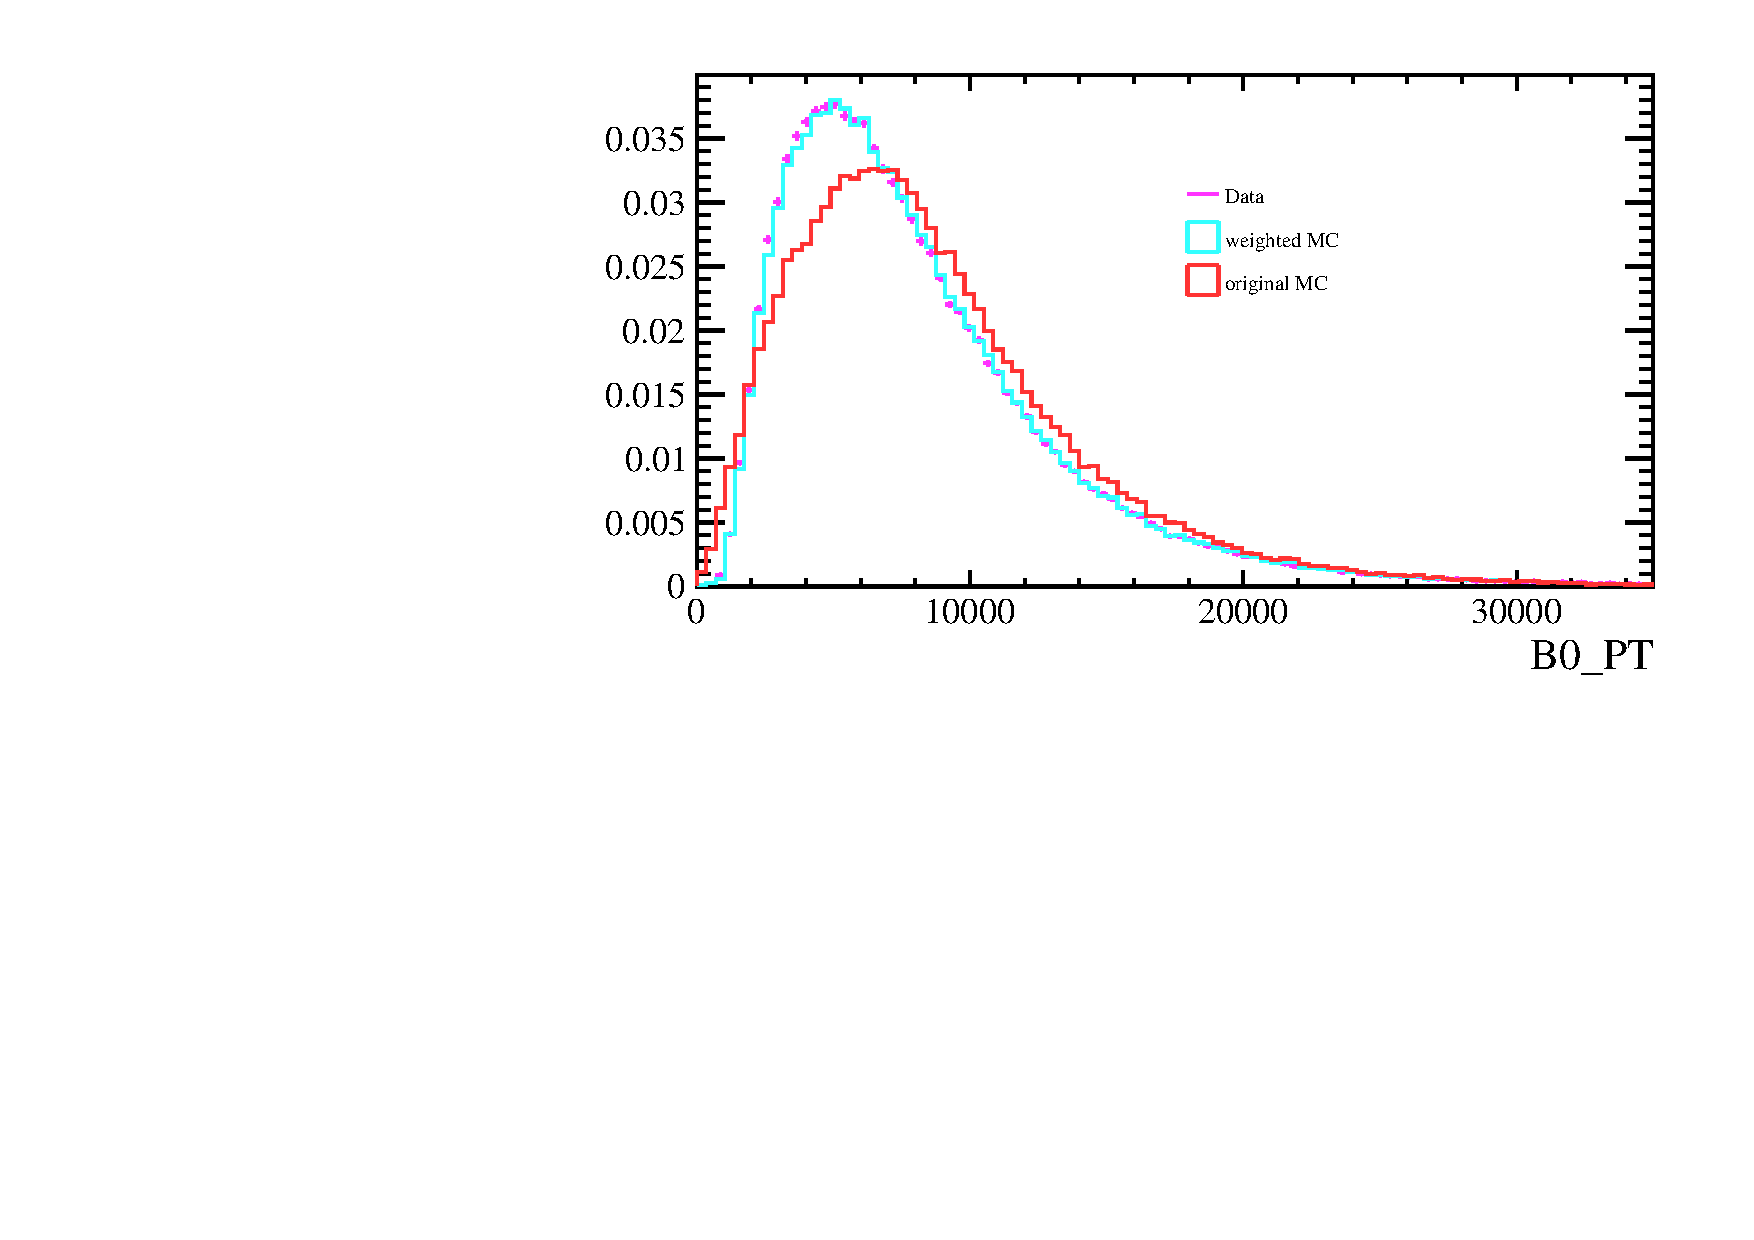
\includegraphics[width=0.8\linewidth]{figures/B0_PT}
   \caption{Result after applieng the weights for the transversal momentum of the $B$ meson (B0\_PT) in MeV.}
  \end{figure}


\end{frame}

%------------------------------------------------------------------------------


\section{RooMCMarkovChain}

%------------------------------------------------
%\subsection{Monte Carlo Markov Chain} % Sections can be created in order to organize your presentation into discrete blocks, all sections and subsections are automatically printed in the table of contents as an overview of the talk
%------------------------------------------------

\begin{frame}
 \frametitle{Monte Carlo Markov Chain}
 A Markov Chain is a random process which undergoes several states. \\
 From each state there is a probability distribution to change into another state or to stay. \\
 Most important is the asumption that every next step just depends on the current state.
 \begin{figure}
  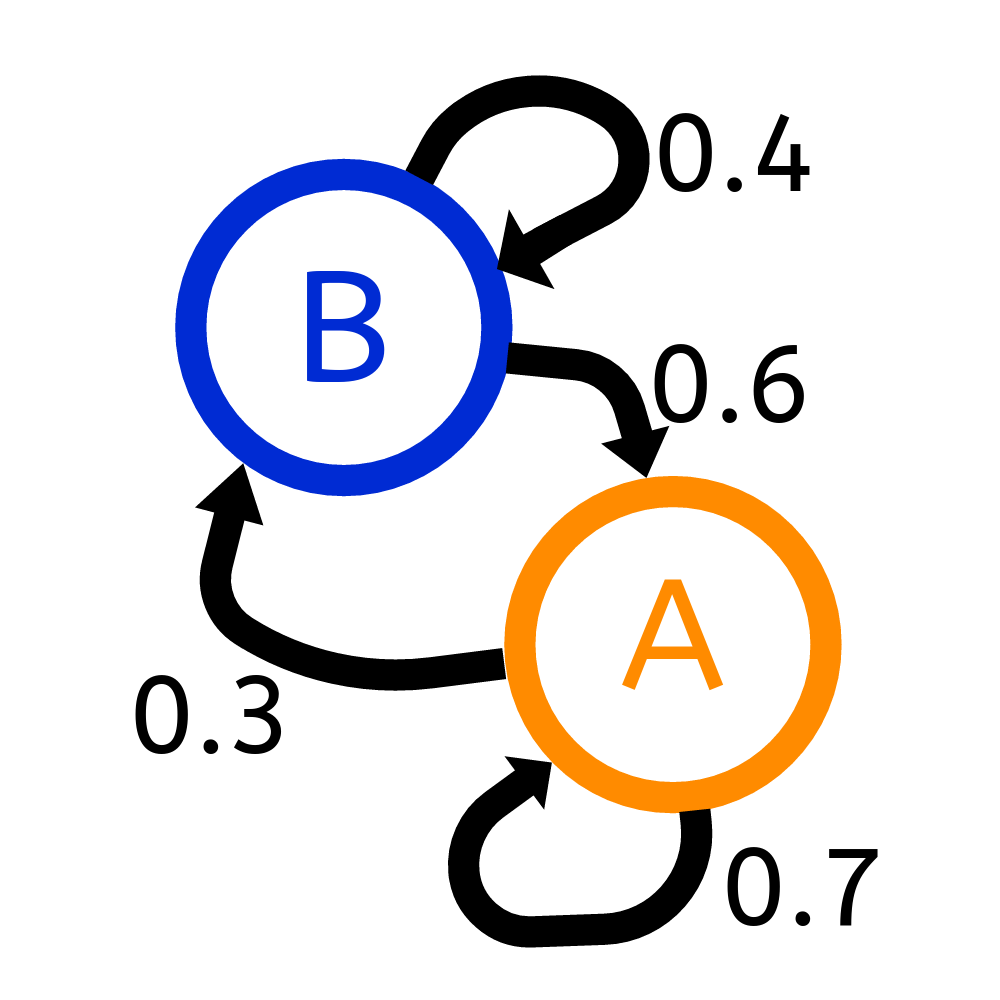
\includegraphics[width=0.3\linewidth]{figures/MCMC_Chain}
  \caption{Example of states and probabilities of states in a Markov Chain}
 \end{figure}
\end{frame}

%--------------------------------------------------------------

%\subsection{Algorithm}


\begin{frame}
 \frametitle{Metropolis-Hastings}
 \begin{itemize}
  \item Current state $x$ is proposed to move to $y$
  \item Calculate Hastings ratio: \\
        \begin{align}
         r(x,y) = \frac{h(y) \cdot q(y,x)} {h(x) \cdot q(x,y)} \label{eq:r(x,y)}
        \end{align}
  \item Where $q(x,\cdot)$ is the conditional probability density \\
        and $h$ is the unnormalized density of the specified distribution
  \item Accept the proposed move to $y$ with the probability: \\
        \begin{align}
         a(x,y) = min(1,r(x,y)).
        \end{align}
 \end{itemize}
 % note that if h(x) = 0 r is undefined so the strting point has to fullfill that condition
 % if y is a bad point with h(y) = 0 for example outside the borders r =0 and the point gets rejected automatically
\end{frame}


%-----------------------------------------------------------
\begin{frame}
 \frametitle{The algorithm}
 \begin{figure}
  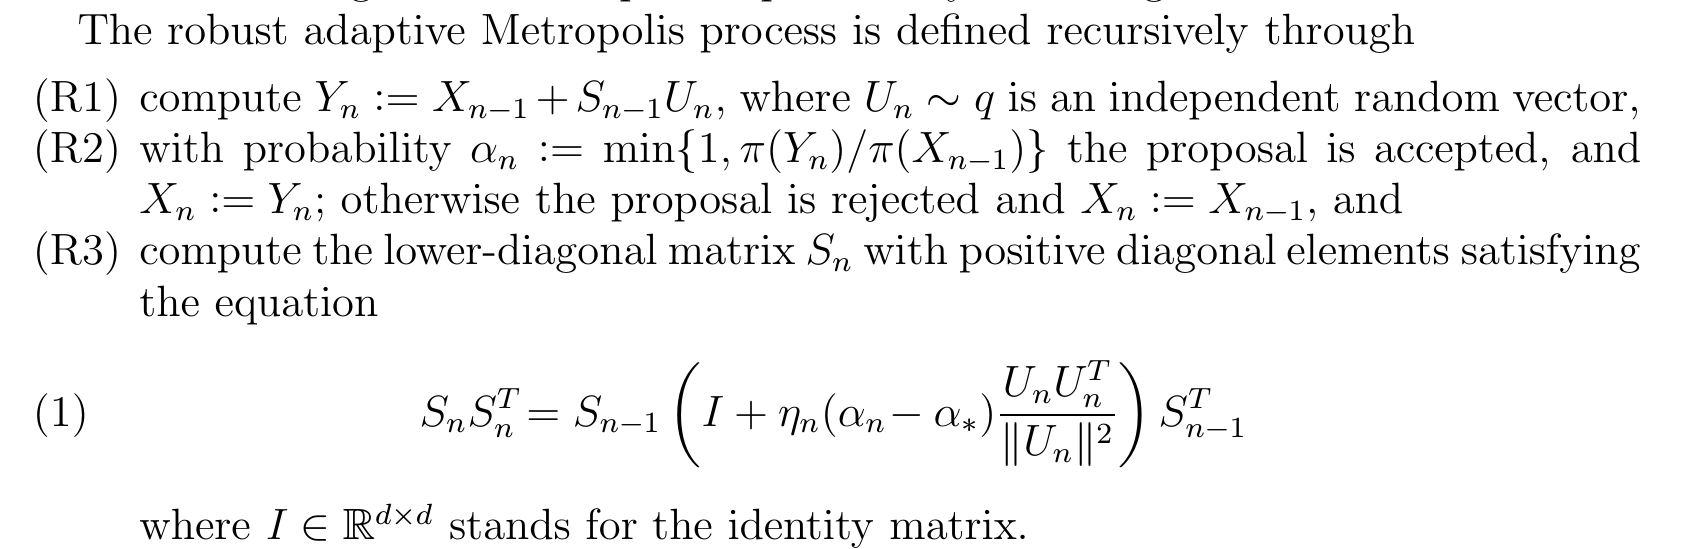
\includegraphics[width=1.0\linewidth]{figures/Metropolis}
  \caption{arXiv: 1011.4381v2}
 \end{figure}
% Rahmen um Bild
 Here $Y_n$ is the next state and $X_{n-1}$ is the current state. \\
 The $S$-maxtrix determs the direction and step size of the next step. \\
 % alpha star is the forced acceptance rate, a good value is 0.234  determed by experience
\end{frame}

%\subsection{Example}

\begin{frame}
 \frametitle{Example}
 fitting the folowing pdf:
 \begin{align}
  \frac{1}{\sqrt{2 \pi \sigma_1^2}} e^{- \frac{(x-\mu_1)^2}{2 \sigma_1^2}} + f \cdot  \frac{1}{\sqrt{2 \pi \sigma_2^2}} e^{- \frac{(x-\mu_2)^2}{2 \sigma_2^2}}
 \end{align}

\end{frame}

%-----------------------------------------------------------
\begin{frame}
 \frametitle{Example}
 \begin{figure}
  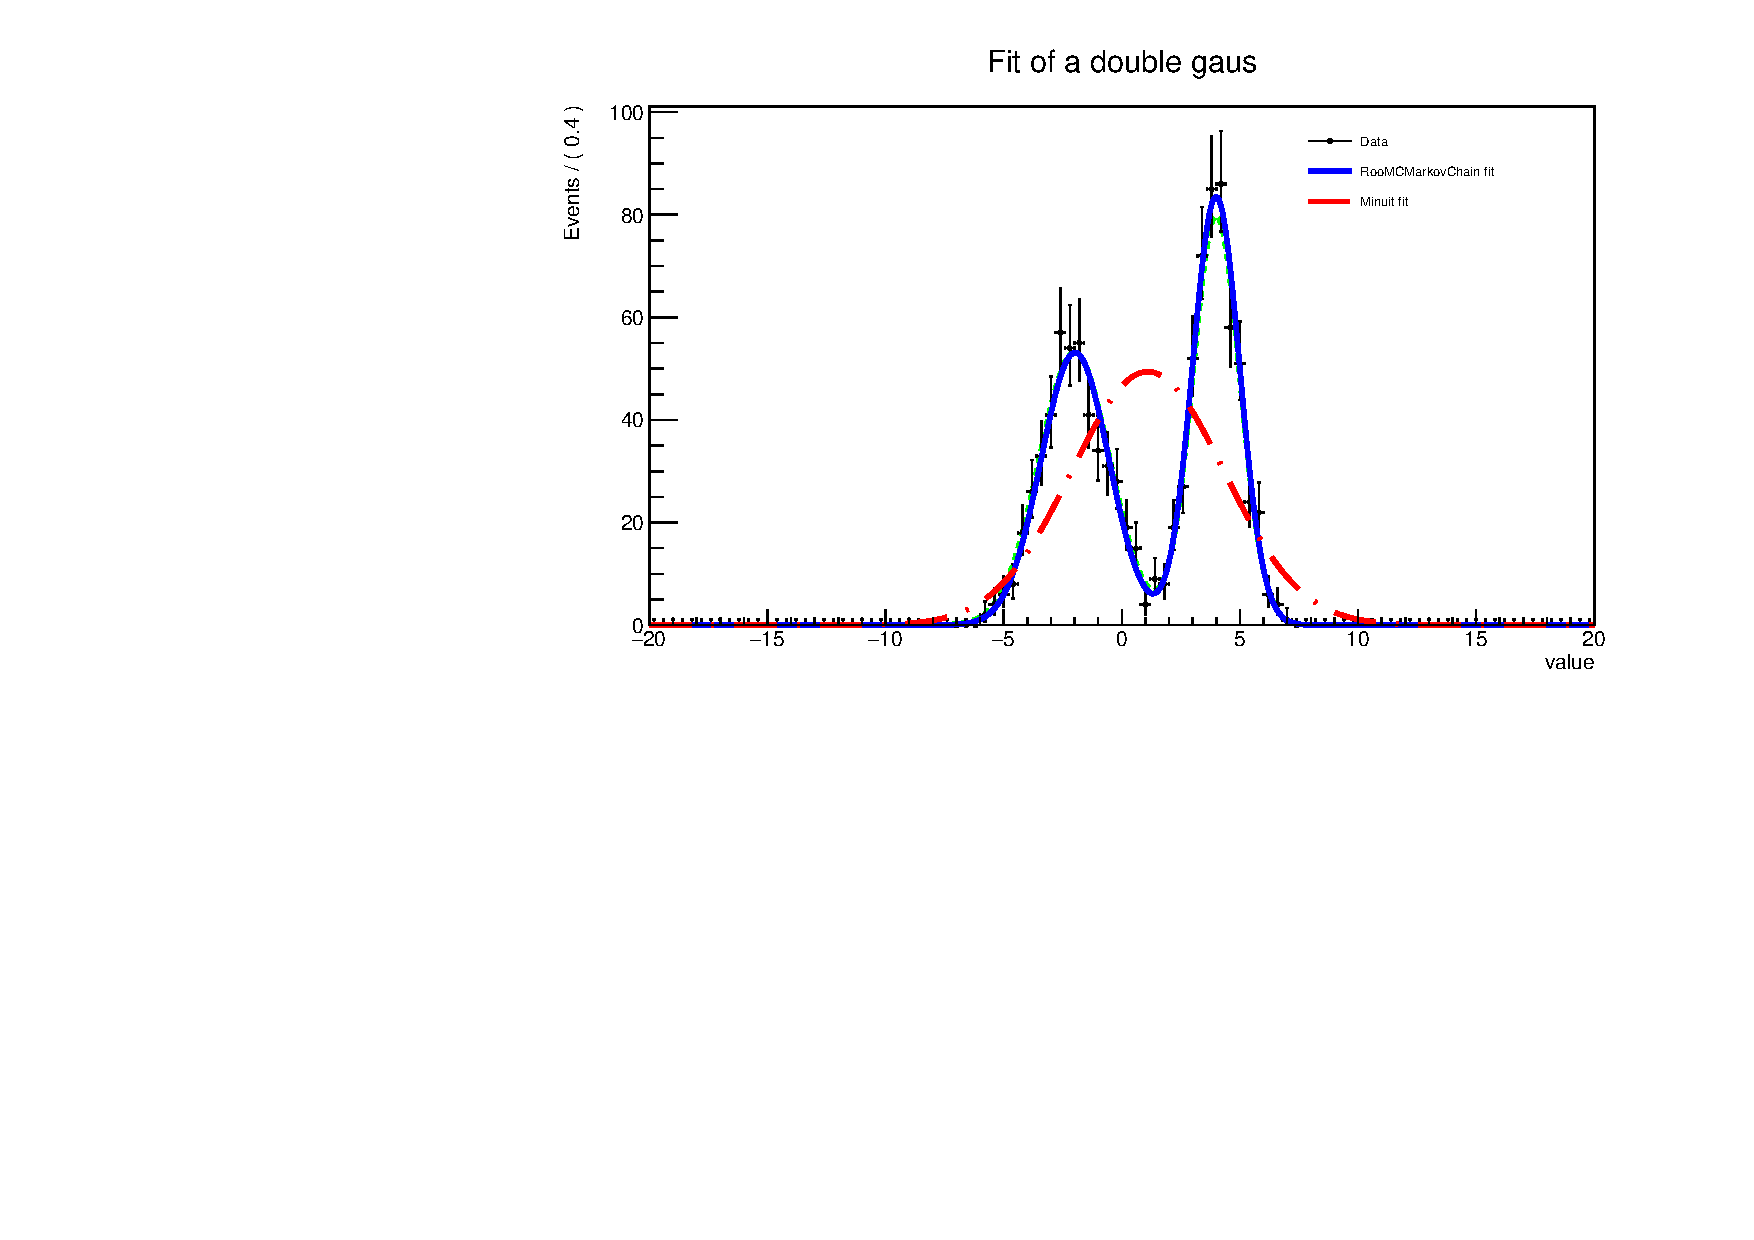
\includegraphics[width=1.0\linewidth]{figures/twogausFit}
  \caption{Fit of a double gaus}
 \end{figure}
\end{frame}

%-----------------------------------------------------------


%\subsection{Features}

%-----------------------------------------------------------
\begin{frame}
 \frametitle{Features}
 \begin{itemize}
  \item The constructor behaves like the RooMinuit constructor RooMCMC(RooAbsReal *negativeloglikelihood)
  \item then mcmc performes the walk and error calculation
  \item RooMCMarkovchain.\textbf{mcmc}(\textbf{int} npoints, \textbf{int} cutoff, \textbf{string} errorstrategy)
  \item there are two errorstategies: "gaus" for syemtric errors and "interval" for asymetric ones
  \item The terminal output is similar to the one of Minuit. It first prints the parameters with errors and then the correlation coefficients.
 \end{itemize}
\end{frame}

%-----------------------------------------------------------
\begin{frame}
 \frametitle{Features}
 \begin{itemize}
  \item To look at the profile of the nll one can use:
  \item TGraph *profile = \textbf{getProfile}(\textbf{string} name, \textbf{bool} cutoff)
  \item with cutoff bool one can include or exclude the cutoff points
 \end{itemize}

 \begin{figure}
  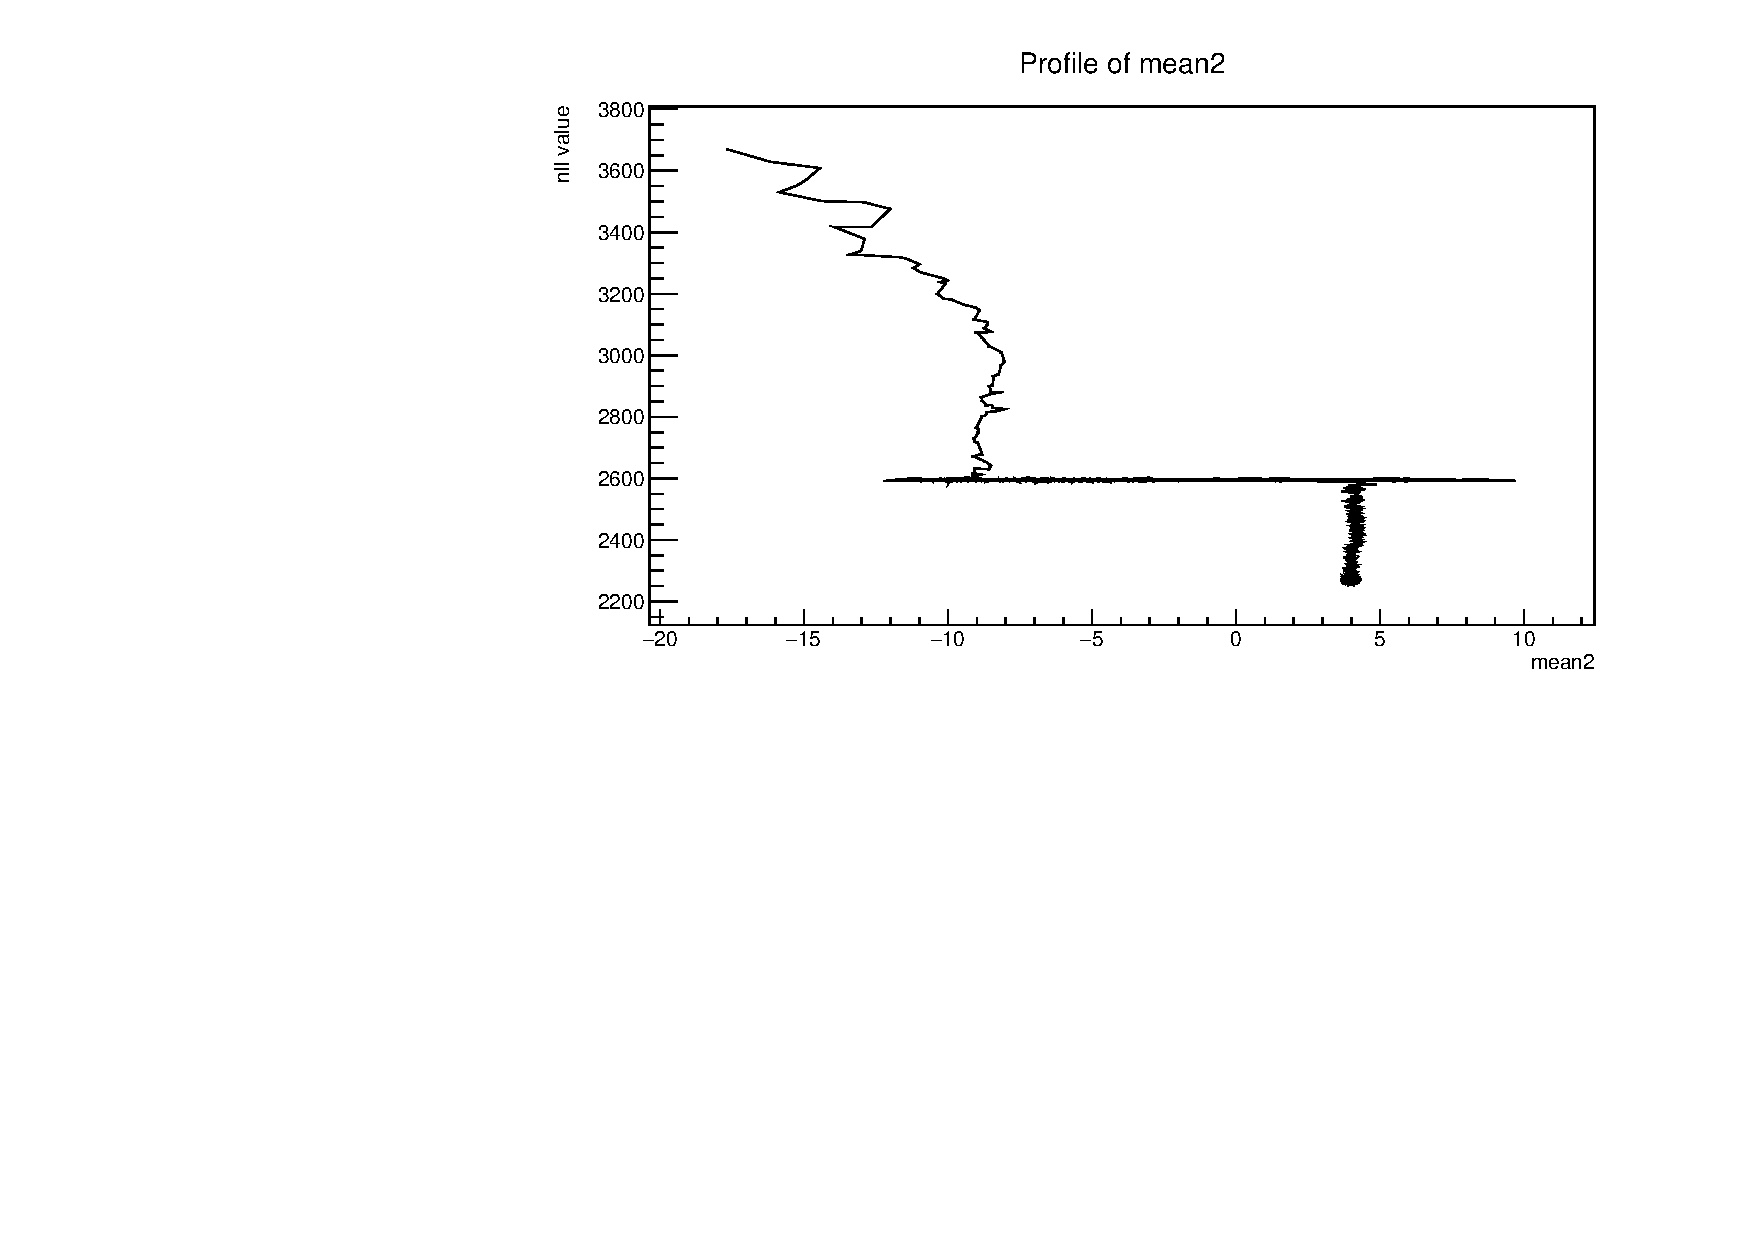
\includegraphics[width=0.8\linewidth]{figures/profile_mean2}
  \caption{Profile from the mean of the second gaus}
 \end{figure}

\end{frame}

%-----------------------------------------------------------
\begin{frame}
 \frametitle{Features}
 \begin{itemize}
  \item It is very important to look at the walk distribution, to check if the cutoff is well placed:
  \item TMultiGraph *walkdis = \textbf{getWalkDis}(\textbf{string} name, \textbf{bool} cutoff)
 \end{itemize}

 \begin{figure}
  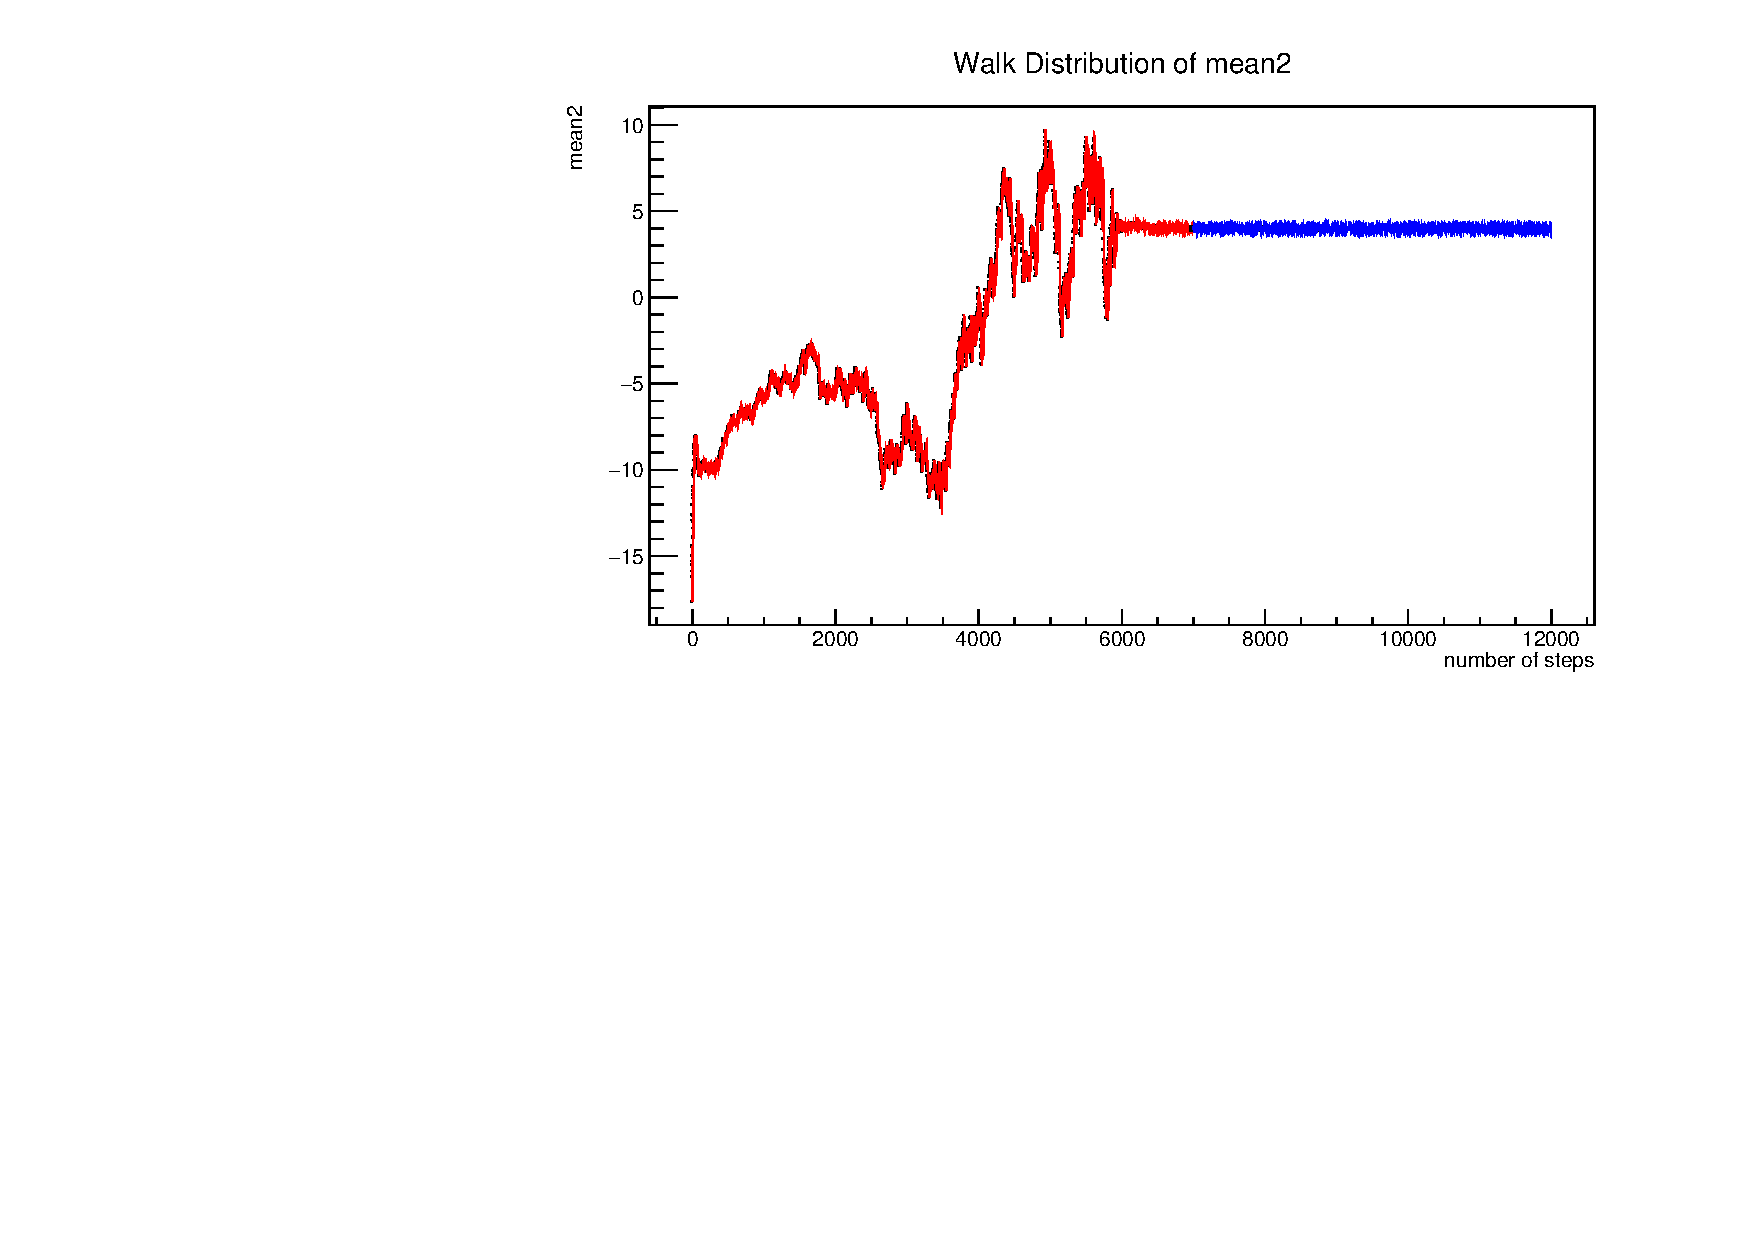
\includegraphics[width=0.8\linewidth]{figures/walkdis_mean2}
  \caption{Walk distribution from the mean of the second gaus}
 \end{figure}

\end{frame}

\begin{frame}
 \frametitle{Features}
 \begin{itemize}
  \item It is also possible to get a histogram of the walk distribution, to check if the errors a symetric or asymetric.
  \item TH1F *walkdishis = \textbf{getWalkDisHis}(\textbf{string} name, \textbf{int} xbins, \textbf{bool} cutoff)
 \end{itemize}

 \begin{figure}
  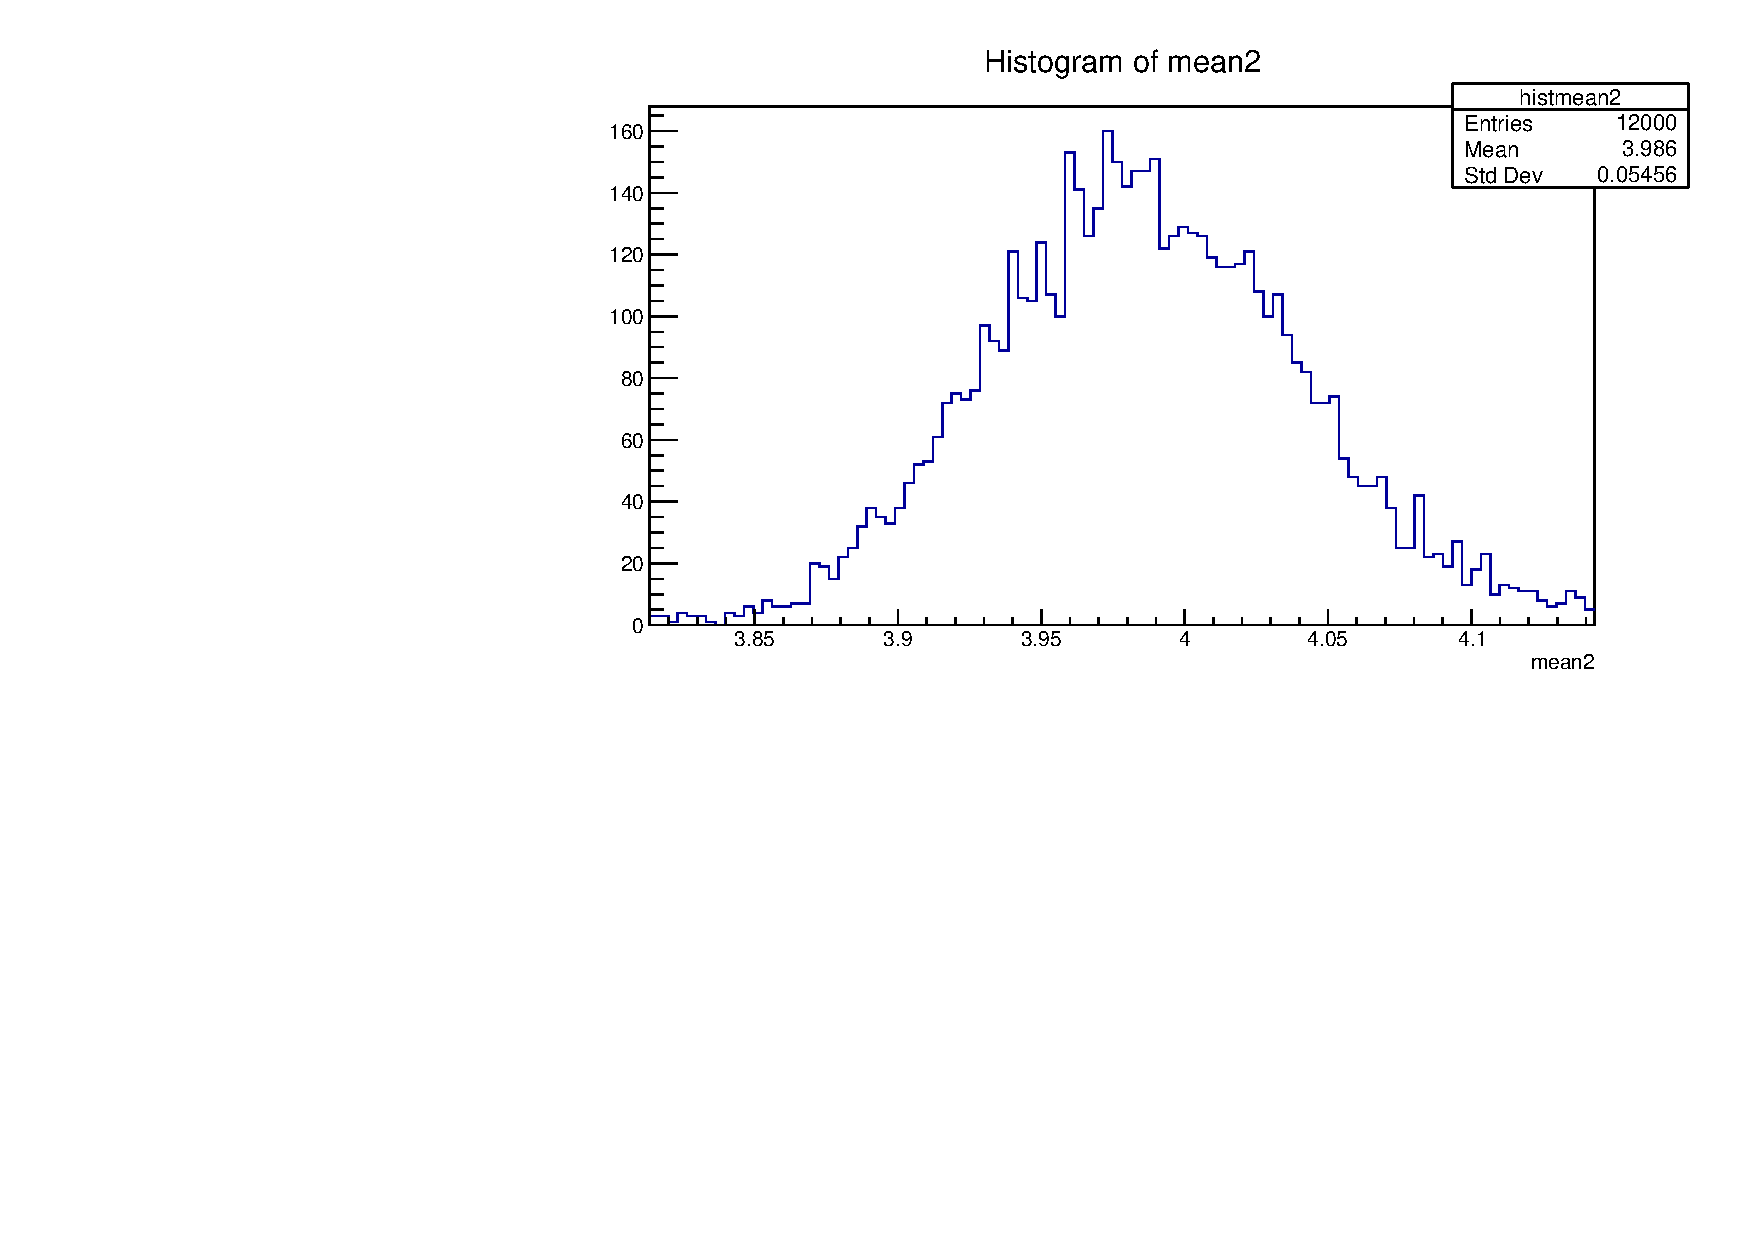
\includegraphics[width=0.8\linewidth]{figures/walkdishis_mean2}
  \caption{Histogram from the walk distribution of the mean of the second gaus}
 \end{figure}

\end{frame}

\begin{frame}
 \frametitle{Features}
 \begin{itemize}
  \item To check for correlations between parameters one can create a cornerplot between them.
  \item TH2D *corner = \textbf{getCornerPlot}(\textbf{string} name1, \textbf{string} name2, \textbf{int} nbinsx, \textbf{int} nbinsy, \textbf{bool} cutoff)
 \end{itemize}

 \begin{figure}
  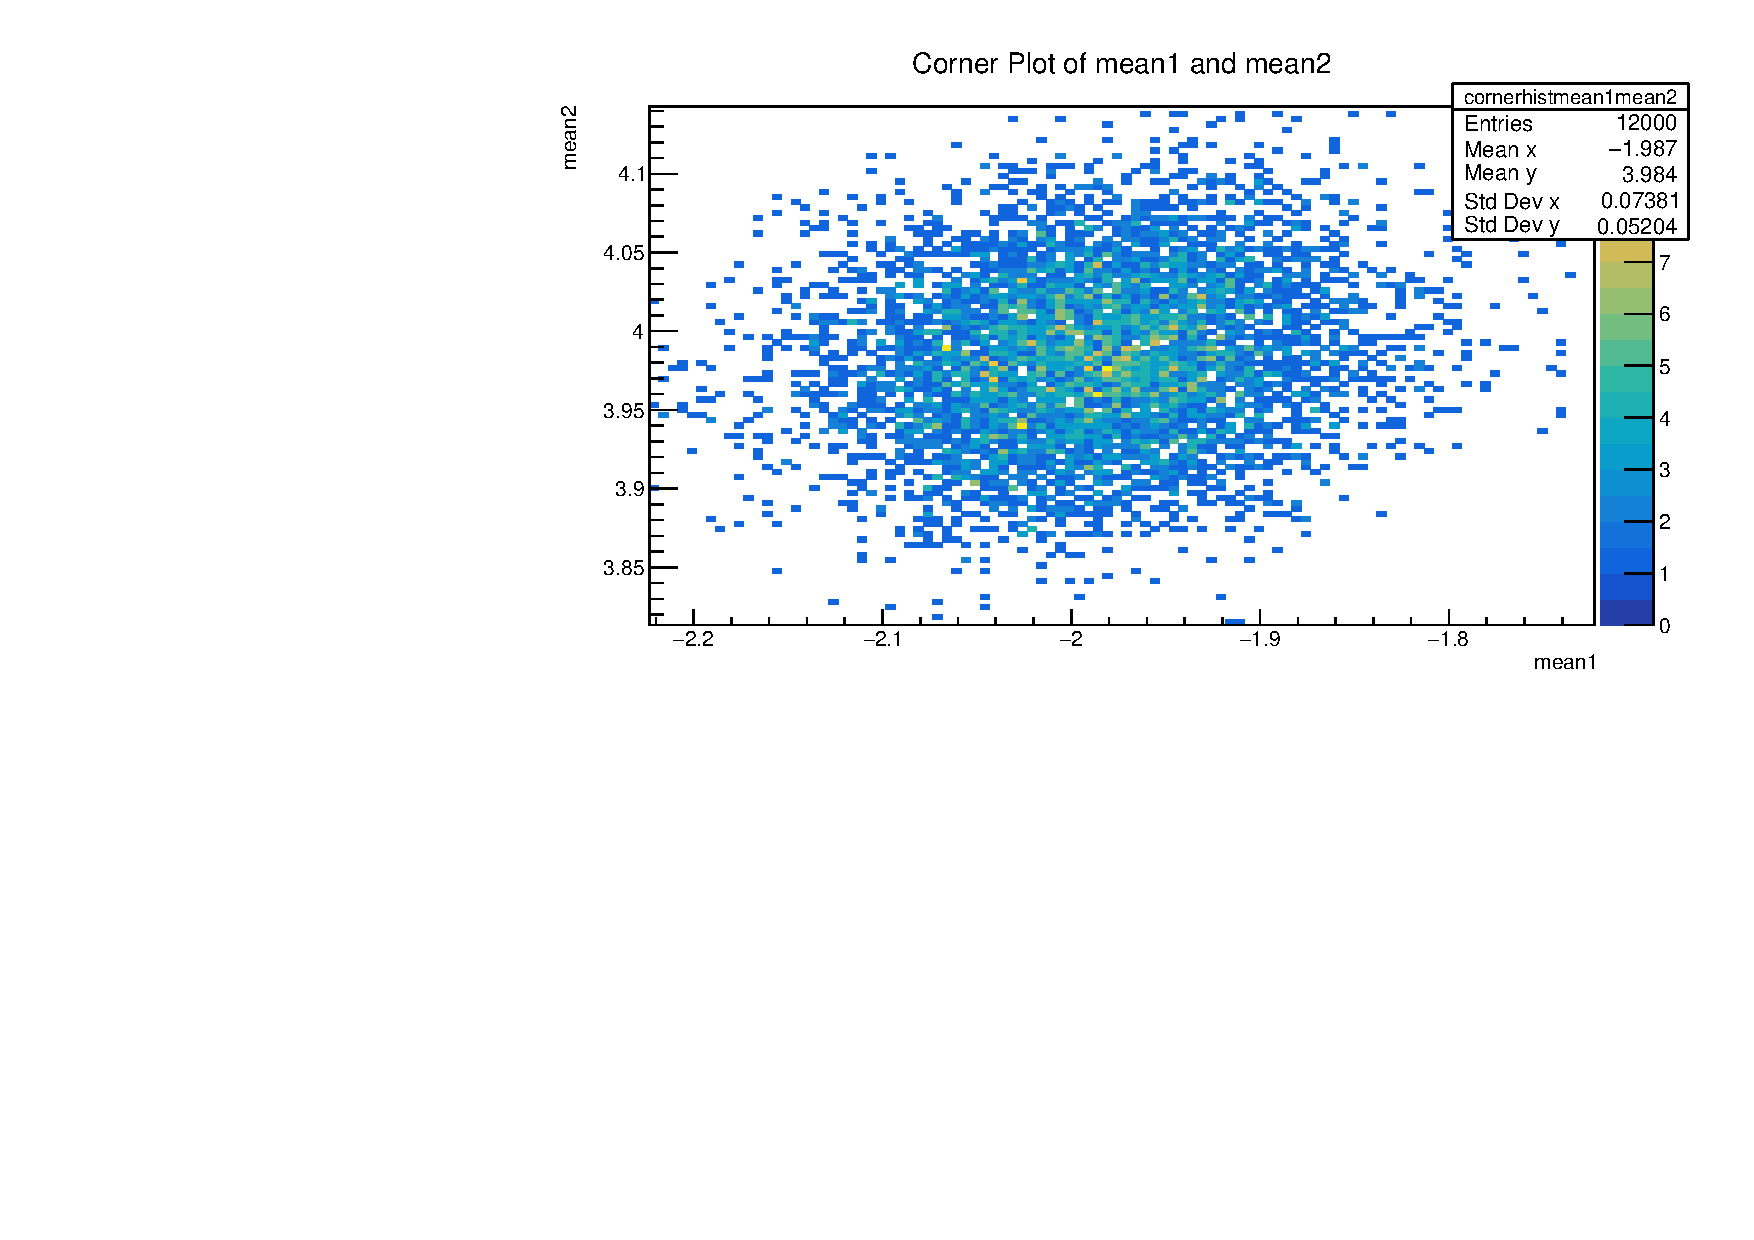
\includegraphics[width=0.8\linewidth]{figures/corner_mean1_mean2}
  \caption{Cornerplot between the mean values of the two gaus.}
 \end{figure}

\end{frame}

%-----------------------------------------------------------
\begin{frame}
 \frametitle{Features}
 \begin{itemize}
  \item Now to put everything together:
  \item \textbf{saveCornerPlotAs}(\textbf{string} picname)
  \item It saves a picture with a histogram of each parameter plus a correlation plot with each parameter pair.
  \item One can see directly if there is any correlation and if errors a symetric or asymetric
 \end{itemize}




\end{frame}

%----------------------------------------------------------------------------------------

\begin{frame}
 \frametitle{Features}

 \begin{figure}
  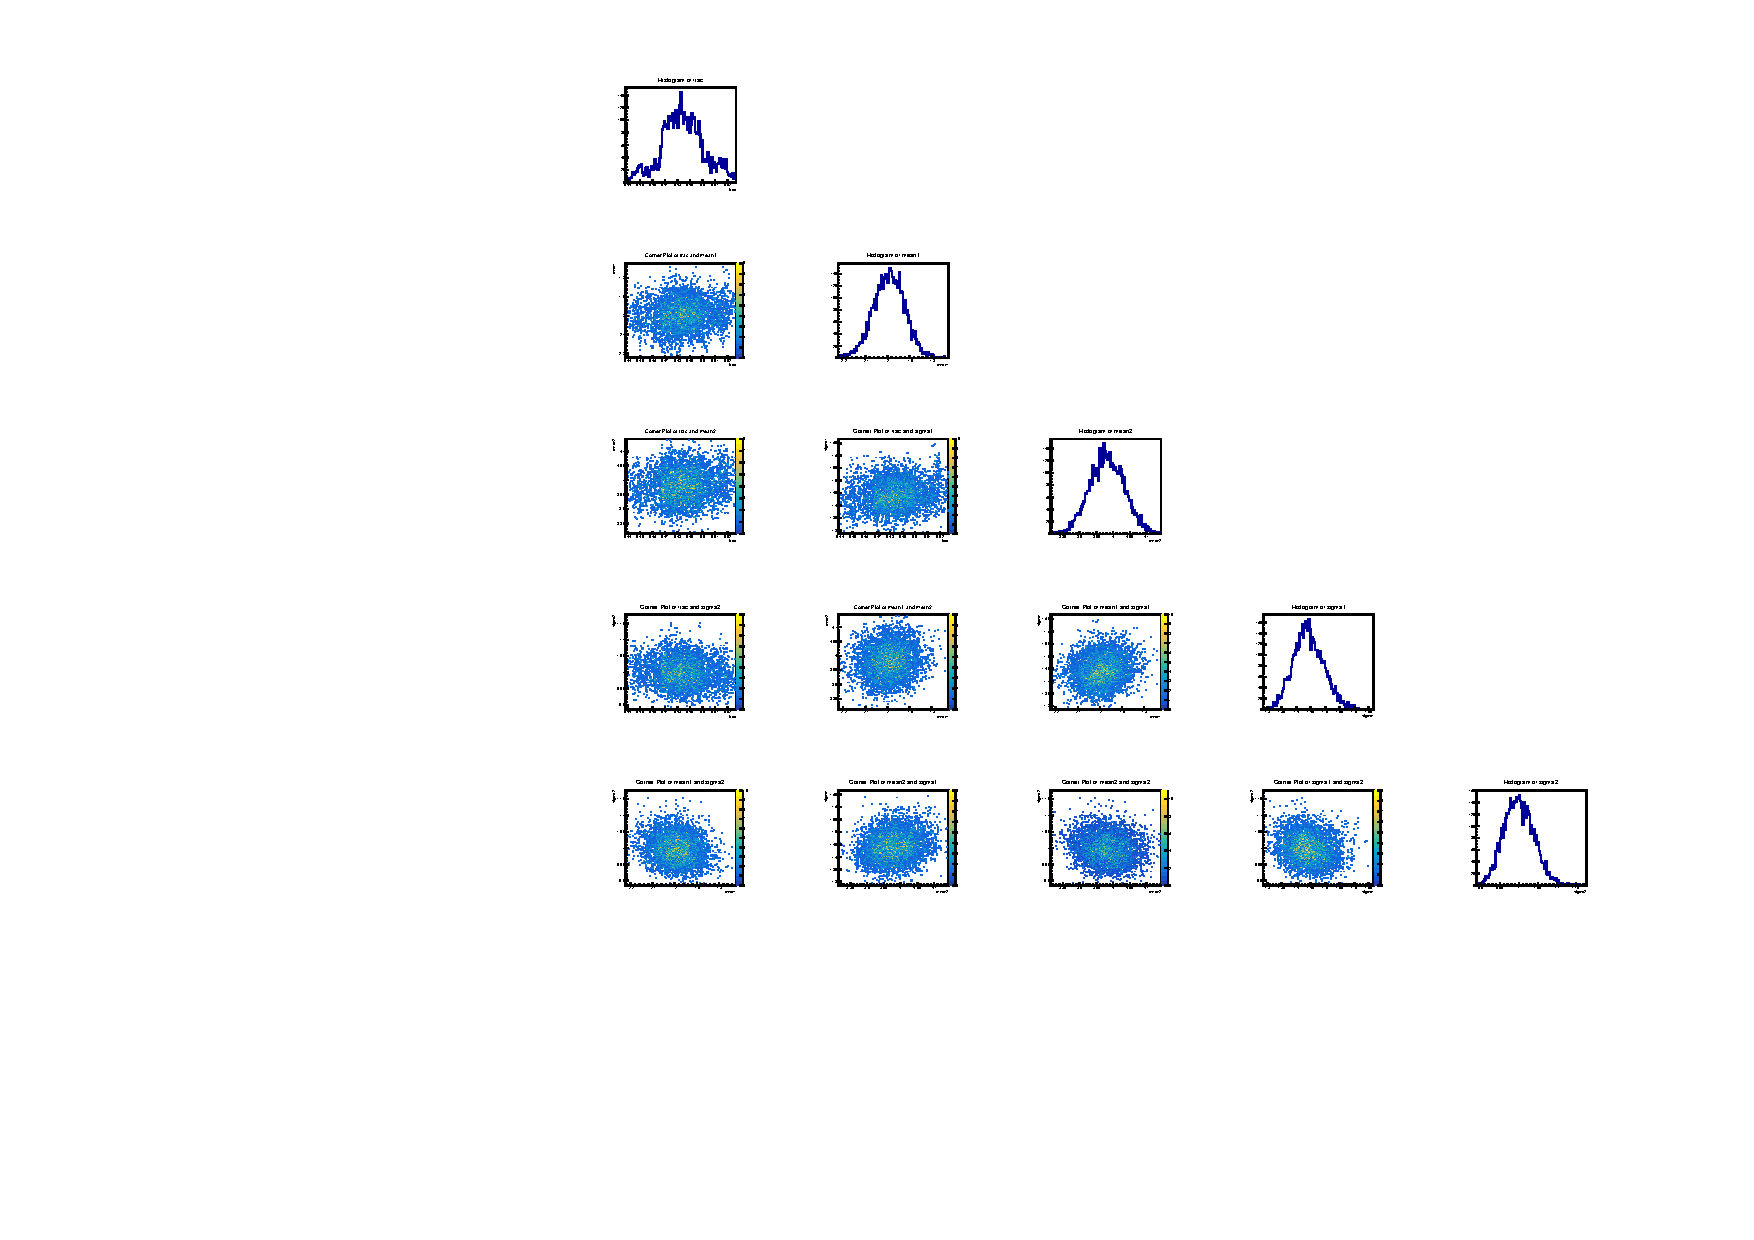
\includegraphics[width=0.8\linewidth]{figures/twogausCorner}
  \caption{Corner Plot of the double gaus fit}
 \end{figure}

\end{frame}

\begin{frame}
 \frametitle{Interested?}


   \centering Pull Request: https://github.com/root-project/root/pull/1422 \\
    --------------------------------------------------------------------- \\
   \centering E-mail: o.dahme@cern.ch

\end{frame}

\begin{frame}
 \frametitle{Summary}

The RooMCMarkovChain fitting routine is currently beeing added to the ROOT Data analysis framework. \\
 The best algorithm uBoost from the boost decision tree test will be used to find future $B \rightarrow K^* \mu \mu$ decays. \\
 The rewighting done in this thesis will be used for the future analysis of the $B \rightarrow K^* \mu \mu$ in the current LHCb data.

\end{frame}



%
%
% \section{Backup}
%
% \begin{frame}
%  \frametitle{Example}
%  fitting the folowing pdf:
%  \begin{align}
%   \sum_{i = 1}^{3} \frac{1}{\sqrt{2 \pi \sigma_i^2}} e^{- \frac{(x-\mu_i)^2}{2 \sigma_i^2}} + \sum_{j=1}^{6} \left(   \pi \sigma_j \left[ 1 + \left( \frac{x - \mu_j}{\sigma_j}  \right)^2  \right] \right)^{-1}
%  \end{align}
%
% \end{frame}
%
% %-----------------------------------------------------------
% \begin{frame}
%  \frametitle{Example}
%  \begin{figure}
%   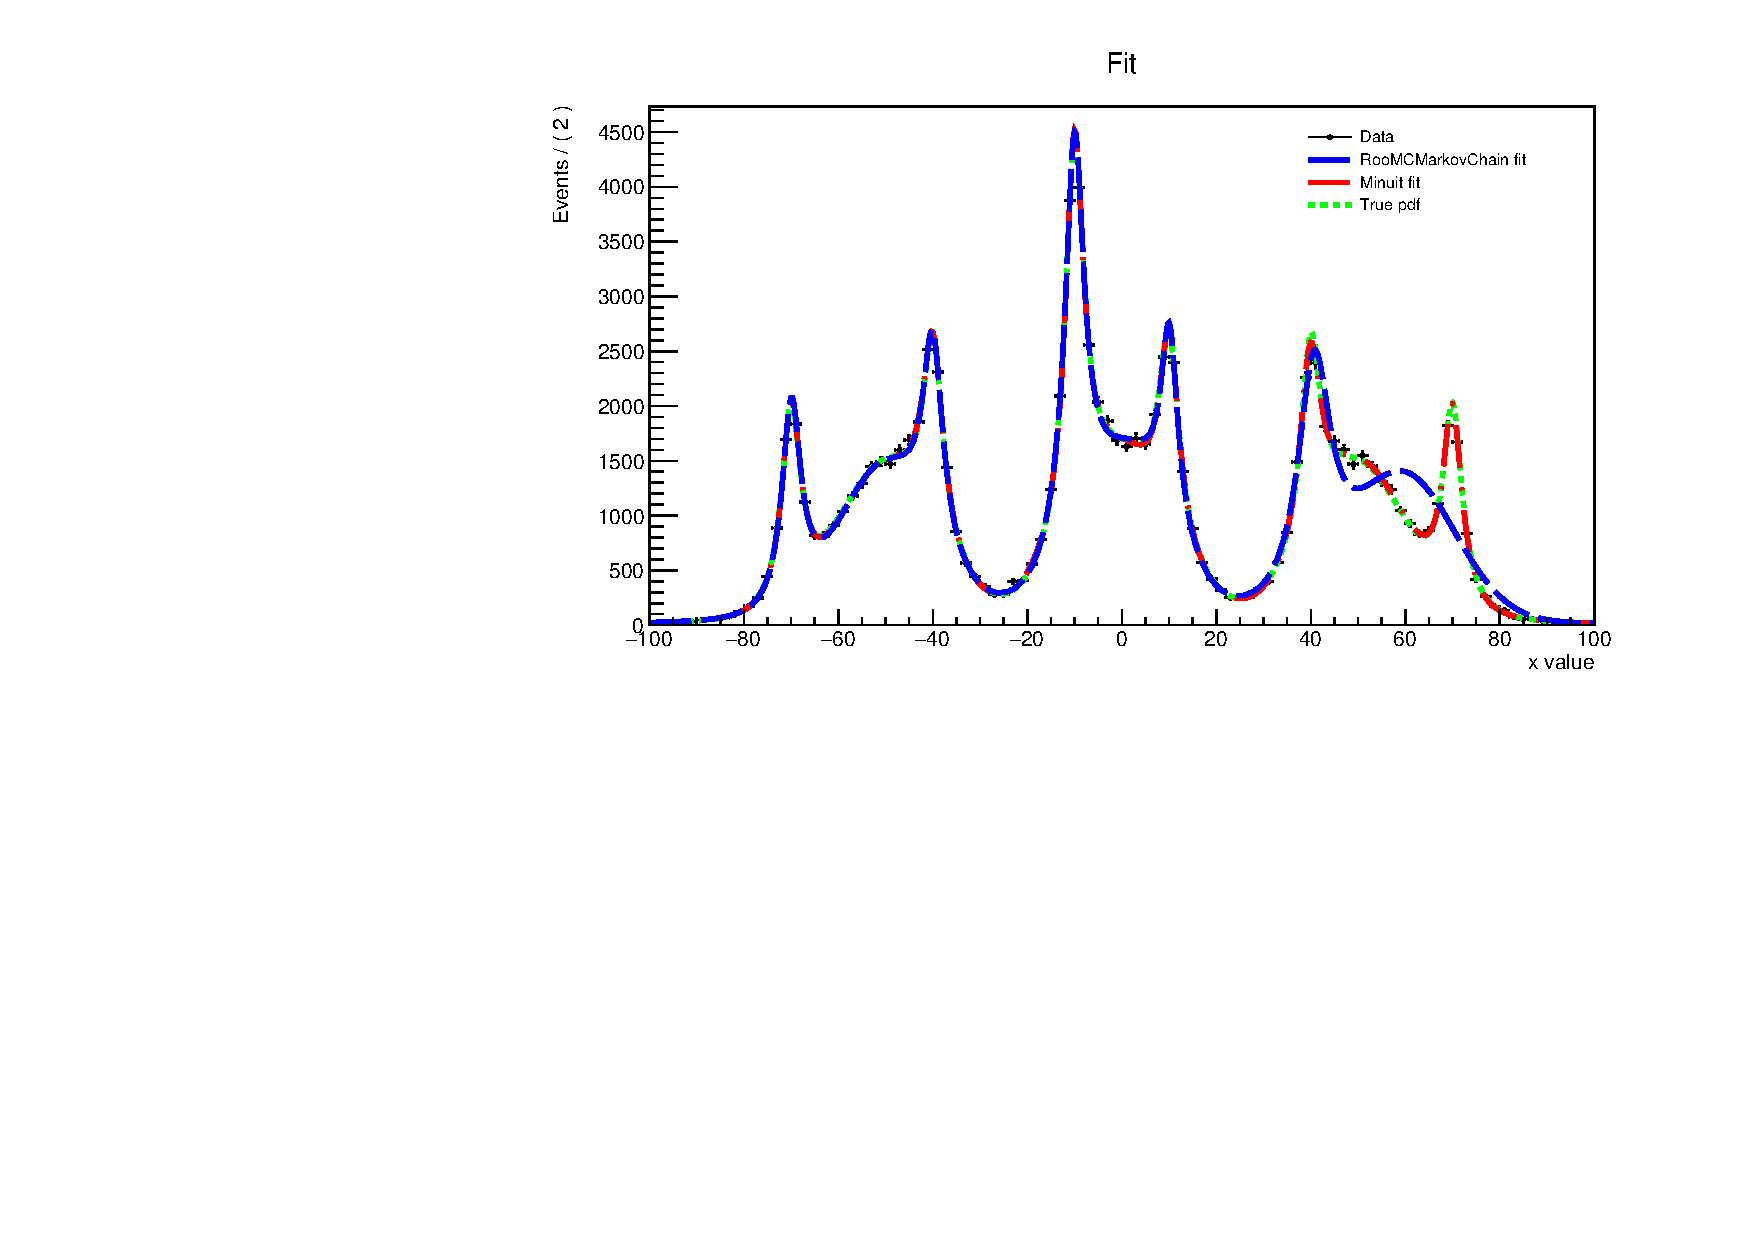
\includegraphics[width=1.0\linewidth]{figures/fit_result_dim0}
%   \caption{Fit of 6 Breit Wigners on top of 3 Gaus.}
%  \end{figure}
% \end{frame}
%
% %-----------------------------------------------------------
%
%
% %-----------------------------------------------------------
% \begin{frame}
%  \frametitle{Features}
%  \begin{itemize}
%   \item The constructor behaves like the RooMinuit constructor
%   \item RooMCMC(negativeloglikelihood)
%   \item then mcmc performes the walk and error calculation
%   \item \textbf{mcmc}(\textbf{int} npoints, \textbf{int} cutoff, \textbf{string} errorstrategy)
%   \item there are two errorstategies: "gaus" for syemtric errors and "interval" for asymetric ones
%  \end{itemize}
% \end{frame}
%
% %-----------------------------------------------------------
% \begin{frame}
%  \frametitle{Features}
%  \begin{itemize}
%   \item To look at the profile of the nll one can use:
%   \item \textbf{getProfile}(\textbf{string} name, \textbf{bool} cutoff)
%   \item with cutoff bool one can include or exclude the cutoff points
%  \end{itemize}
%
%  \begin{figure}
%   \includegraphics[width=0.8\linewidth]{figures/profile_mean_bW6}
%   \caption{Profile from the mean of the 6. Breit Wigner.}
%  \end{figure}
%
% \end{frame}
%
% %-----------------------------------------------------------
% \begin{frame}
%  \frametitle{Features}
%  \begin{itemize}
%   \item It is very important to look at the walk distribution, to check if the cutoff is well placed:
%   \item \textbf{getWalkDis}(\textbf{string} name, \textbf{bool} cutoff)
%  \end{itemize}
%
%  \begin{figure}
%   \includegraphics[width=0.8\linewidth]{figures/walkdis_mean_bW6}
%   \caption{Walk distribution from the mean of the 6. Breit Wigner.}
%  \end{figure}
%
% \end{frame}
%
%


\end{document}
